\begin{enumerate}[label=\thechapter.\arabic*,ref=\thechapter.\theenumi]

\item An $8$ bit ADC converts analog voltage in the range of $0$ to $+5\, V$ to the corresponding digital code as per the conversion characteristics shown in figure. For $V_{in} = 1.9922\, V$, which of the following digital output, given in hex, is true?

\begin{figure}[!h]
    \centering
    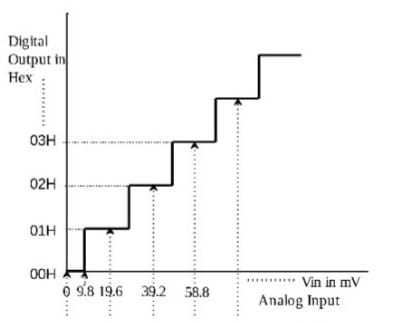
\includegraphics[width=\columnwidth]{2023/EE/40/figs/fig1.jpeg}
    \caption{}
    \label{fig:ADC_gate.ee.23.40}
\end{figure}
\begin{enumerate}[label=(\alph*)]
    \item $64H$
    \item $65H$
    \item $66H$
    \item $67H$
\end{enumerate} \hfill(GATE EE 40)

\solution
\iffalse
\let\negmedspace\undefined
\let\negthickspace\undefined
\documentclass[journal,12pt,twocolumn]{IEEEtran}
\usepackage{cite}
\usepackage{amsmath,amssymb,amsfonts,amsthm}
\usepackage{algorithmic}
\usepackage{graphicx}
\usepackage{textcomp}
\usepackage{xcolor}
\usepackage{txfonts}
\usepackage{listings}
\usepackage{enumitem}
\usepackage{mathtools}
\usepackage{gensymb}
\usepackage{comment}
\usepackage[breaklinks=true]{hyperref}
\usepackage{tkz-euclide} 
\usepackage{listings}
\usepackage{gvv}                                        
\def\inputGnumericTable{}                                
\usepackage[latin1]{inputenc}                            
\usepackage{color}                                       
\usepackage{array}                                       
\usepackage{longtable}                                   
\usepackage{calc}                              
\usepackage{tikz}
\usepackage{multirow}                                    
\usepackage{hhline}                                      
\usepackage{ifthen}                            
\usepackage{caption}
\usepackage{lscape}
\usepackage{amsmath}
\newtheorem{theorem}{Theorem}[section]
\newtheorem{problem}{Problem}
\newtheorem{proposition}{Proposition}[section]
\newtheorem{lemma}{Lemma}[section]
\newtheorem{corollary}[theorem]{Corollary}
\newtheorem{example}{Example}[section]
\newtheorem{definition}[problem]{Definition}
\newcommand{\BEQA}{\begin{eqnarray}}
\newcommand{\EEQA}{\end{eqnarray}}
\newcommand{\define}{\stackrel{\triangle}{=}}
\theoremstyle{remark}
\newtheorem{rem}{Remark}

\begin{document}

\bibliographystyle{IEEEtran}
\vspace{3cm}

\title{NCERT Math 11.9.2 Q8}
\author{EE23BTECH11009 - AROSHISH PRADHAN$^{*}$% <-this % stops a space
}
\maketitle
\newpage
\bigskip
\textbf{Question:} An $8$ bit ADC converts analog voltage in the range of $0$ to $+5\, V$ to the corresponding digital code as per the conversion characteristics shown in figure. For $V_{in} = 1.9922\, V$, which of the following digital output, given in hex, is true?

\begin{figure}[!h]
    \centering
    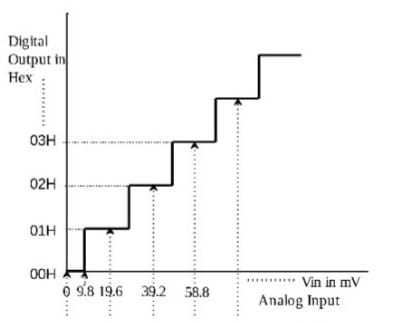
\includegraphics[width=\columnwidth]{2023/EE/40/figs/fig1.jpeg}
    \caption{}
    \label{fig:ADC_gate.ee.23.40}
\end{figure}
\begin{enumerate}[label=(\alph*)]
    \item $64H$
    \item $65H$
    \item $66H$
    \item $67H$
\end{enumerate}

\solution
\fi
\begin{table}[!h]
    \centering
    \resizebox{\columnwidth}{!}{\begin{tabular}{|c|c|c|}
    \hline
       \textbf{Symbol}  & \textbf{Value} & \textbf{Description}\\
    \hline
        $n$  &  $8$ &  Number of bits of ADC\\
    \hline
        $V_{min}$ & $0V$ & Minimum Analog Voltage\\
    \hline
        $V_{max}$ & $5V$ & Maximum Analog Voltage\\
    \hline
        $V_{in}$ & $1.9922 V$ & Input Voltage\\
    \hline
        $V_{out}$ & & Output Voltage\\
    \hline
\end{tabular}
}
    \caption{Given Parameters}
    \label{tab:1_gate.ee.23.40}
\end{table}

Calculating the step-size:
\begin{align}
    \Delta V_{in} &= \frac{V_{max} - V_{min}}{2^n - 1}\\
    &= \frac{5 - 0}{2^8 - 1}\\
    &= \frac{5}{255}\\
   \implies V_{out} &= \frac{V_{in}}{\Delta V_{in}}\\
    &= \frac{1.9922 \times 255}{5}\\
    &= 101.59\\
    &\approx 102_{10}\\
    &= (66)_{H}
\end{align}
$\therefore$ correct answer is option (c).
\begin{figure}[!h]
    \centering
    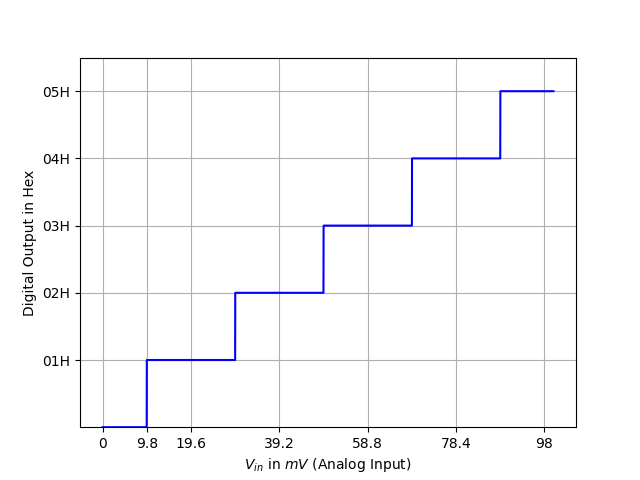
\includegraphics[width=\columnwidth]{2023/EE/40/figs/assign3.png}
    \caption{}
    \label{fig:ADC_plot_gate.ee.23.40}
\end{figure}

\newpage
\item Let x1\brak{t} and x2\brak{t} be two band-limited signals having bandwidth B = $4\pi\times10^3$
rad/s each. In the figure below, the Nyquist sampling frequency, in
rad/s, required to sample y\brak{t}, is
 \begin{circuitikz}
     \draw (0,0) node[left] {$x_1(t)$} to (0.8,0);
     \draw (0,-1) node[left] {$x_2(t)$} to (0.8,-1);
     \draw (1,0) circle(0.2);
     \draw (1,0) node {$\times$};
     \draw (1,-1) circle(0.2);
     \draw (1,-1) node {$\times$};
    \draw (1.2,0) to (1.8,0);
    \draw (1.2,-1) to (1.8,-1);
    \draw (1.8,0) to (1.8,-0.3);
    \draw (1.8,-1) to (1.8,-0.7);
    \draw (1.8,-0.5) circle(0.2);
    \draw (1.8,-0.5) node {$+$};
    \draw[->] (1,0.5) to (1,0.2) ;
    \node at (1,0.6) {cos$(4\pi\times10^3t)$};
    \draw[->] (1,-1.5) to (1,-1.2);
    \node at (1,-1.6) {cos$(12\pi\times10^3t)$};
    \draw (2,-0.5) to (2.3,-0.5);
    \node at (2.6,-0.5) {y(t)};
     
     
\end{circuitikz}
 \\
\begin{enumerate}[label=(\alph*)]
    \item $20\pi\times10^3$
    \item $40\pi\times10^3$
    \item $8\pi\times10^3$
    \item $32\pi\times10^3$
\end{enumerate} \hfill(GATE EC 50)


\solution
\iffalse
\let\negmedspace\undefined
\let\negthickspace\undefined
\documentclass[journal,12pt,twocolumn]{IEEEtran}
\usepackage{cite}
\usepackage{amsmath,amssymb,amsfonts,amsthm}
\usepackage{algorithmic}
\usepackage{graphicx}
\usepackage{textcomp}
\usepackage{xcolor}
\usepackage{txfonts}
\usepackage{listings}
\usepackage{enumitem}
\usepackage{mathtools}
\usepackage{gensymb}
\usepackage{comment}
\usepackage[breaklinks=true]{hyperref}
\usepackage{tkz-euclide} 
\usepackage{listings}
\usepackage{gvv}                                        
\def\inputGnumericTable{}                                 
\usepackage[latin1]{inputenc}                         
\usepackage{circuitikz}
\usepackage{color}                                            
\usepackage{array}                                            
\usepackage{longtable}                                       
\usepackage{calc}                                             
\usepackage{multirow} 

\usepackage{hhline}                                           
\usepackage{ifthen}                                           
\usepackage{lscape}


\newtheorem{theorem}{Theorem}[section]
\newtheorem{problem}{Problem}
\newtheorem{proposition}{Proposition}[section]
\newtheorem{lemma}{Lemma}[section]
\newtheorem{corollary}[theorem]{Corollary}
\newtheorem{example}{Example}[section]
\newtheorem{definition}[problem]{Definition}
\newcommand{\BEQA}{\begin{eqnarray}}
\newcommand{\EEQA}{\end{eqnarray}}
\newcommand{\define}{\stackrel{\triangle}{=}}
\theoremstyle{remark}
\newtheorem{rem}{Remark}


\begin{document}
\parindent 0px
\bibliographystyle{IEEEtran}

\title{GATE 2023 - EC 50}
\author{EE23BTECH11220 - R.V.S.S Varun$^{}$% <-this % stops a space
}
\maketitle
\newpage
\bigskip

\renewcommand{\thefigure}{\theenumi}
\renewcommand{\thetable}{\theenumi}
\section*{Question}

Let $x_1\brak{t}$ and $x_2\brak{t}$ be two band-limited signals having bandwidth B = $4\pi\times10^3$
rad/s each. In the figure below, the Nyquist sampling frequency, in
rad/s, required to sample y\brak{t}, is
  \\
  \vspace{25pt}
\begin{figure}[ht]
    \centering
	\begin{circuitikz}
    \begin{circuitikz}
     \draw (0,0) node[left] {$x_1(t)$} to (0.8,0);
     \draw (0,-1) node[left] {$x_2(t)$} to (0.8,-1);
     \draw (1,0) circle(0.2);
     \draw (1,0) node {$\times$};
     \draw (1,-1) circle(0.2);
     \draw (1,-1) node {$\times$};
    \draw (1.2,0) to (1.8,0);
    \draw (1.2,-1) to (1.8,-1);
    \draw (1.8,0) to (1.8,-0.3);
    \draw (1.8,-1) to (1.8,-0.7);
    \draw (1.8,-0.5) circle(0.2);
    \draw (1.8,-0.5) node {$+$};
    \draw[->] (1,0.5) to (1,0.2) ;
    \node at (1,0.6) {cos$(4\pi\times10^3t)$};
    \draw[->] (1,-1.5) to (1,-1.2);
    \node at (1,-1.6) {cos$(12\pi\times10^3t)$};
    \draw (2,-0.5) to (2.3,-0.5);
    \node at (2.6,-0.5) {y(t)};
     
     
\end{circuitikz}

	\end{circuitikz}
    \label{fig:EC50.1}
\end{figure} 

    \brak{a} $20\pi\times10^3$\\
    \brak{b} $40\pi\times10^3$\\
    \brak{c} $8\pi\times10^3$\\
    \brak{d} $32\pi\times10^3$   \hfill(GATE EC 50)\\




\fi

\begin{table}[ht]
    \centering
    \begin{tabular}{|c|c|c|}
    \hline
	Symbol &Description&Value \\
        \hline
	$f_1$&Frequency of cos$\brak{4\pi\times10^3}$&$2\times10^3$ \\
        \hline
	$f_2$&Frequency of cos$\brak{12\pi\times10^3}$&$6\times10^3$ \\
	\hline
	$f_m$&Maximum frequency of the output signal&- \\
	\hline
	 $\omega_{m}$&-&$2\pi f_m$ \\
         \hline
	 $\omega_{s}$&Nyquist sampling rate&$2\omega_m$ \\
         \hline
    \end{tabular}
 
    \caption{Table of parameters}
    \label{tab:EC50.1}
\end{table}


\begin{figure}[ht]
    \centering
	
    \begin{circuitikz}
    \draw[->] (-5,0) to (5,0);
    \draw[->] (0,-1) to (0,5);
    \draw (-3,0) to (0,3);
    \draw (0,3) to (3,0);
    \draw (-3,-0.5) node {$-2\times10^3$};
    \draw (3,-0.5) node {$2\times10^3$};
    \draw (0,5.5) node {$X_{1}\brak{f}$};

\end{circuitikz}

	
    \label{fig:EC50.2}
\end{figure} 


\begin{figure}[ht]
    \centering
	
    \begin{circuitikz}
    \draw[->] (-5,0) to (5,0);
    \draw[->] (0,-1) to (0,5);
    \draw (-3,0) to (0,3);
    \draw (0,3) to (3,0);
    \draw (-3,-0.5) node {$-2\times10^3$};
    \draw (3,-0.5) node {$2\times10^3$};
    \draw (0,5.5) node {$X_{2}\brak{f}$};
\end{circuitikz}

	
    \label{fig:EC50.3}
\end{figure} 

 From question figure ,
\begin{align}
y\brak{t}=x_1\brak{t}\times cos\brak{4\pi\times10^3t}+x_2\brak{t}\times cos\brak{12\pi\times10^3t}
\end{align}
\begin{align}
	y\brak{t}=y_1\brak{t}+y_2\brak{t}\\
	Y\brak{f}=Y_1\brak{f}+Y_2\brak{f}\label{EC50.1}
\end{align}
\begin{align}
	Y_1\brak{f}&=X_1\brak{f}*\frac{1}{2}[\delta\brak{f-f_1}+\delta\brak{f+f_1}]\\
	      &=\frac{1}{2}[X_1\brak{f-f_1}+X_1\brak{f+f_1}]
\end{align}
\begin{figure}[ht]
    \centering
	
    \begin{circuitikz}[scale=0.8]
    \draw[->] (-5,0) to (5,0);
     \draw[->] (0,-1) to (0,4);
     \draw (-2,0) to (-1,2);
     \draw (-1,2) to (0,0);
     \draw (0,0) to (1,2);
     \draw (1,2) to (2,0);
     \draw (-2,-0.5) node {$-4\times10^3$};
     \draw (2,-0.5) node {$4\times10^3$};
    \draw (0,4.5) node {$Y_{1}\brak{f}$};
\end{circuitikz}

	
    \label{fig:EC50.4}
\end{figure} 

\begin{align}
	Y_2\brak{f}&=X_2\brak{f}*\frac{1}{2}[\delta\brak{f-f_2}+\delta\brak{f+f_2}]\\ 
	&=\frac{1}{2}[X_2\brak{f-f_2}+X_2\brak{f+f_2}]
\end{align}
\clearpage

\begin{figure}[ht]
    \centering
	
    \begin{circuitikz}[scale=0.8]
    \draw[->] (-5,0) to (5,0);
     \draw[->] (0,-1) to (0,4);
     \draw (-4,0) to (-3,2);
     \draw (-3,2) to (-2,0);
     \draw (2,0) to (3,2);
     \draw (3,2) to (4,0);
     \draw (-4,-0.5) node {$-8\times10^3$};
     \draw (-2,-0.5) node {$-4\times10^3$};
     \draw (2,-0.5) node {$-4\times10^3$};
     \draw (4,-0.5) node {$-8\times10^3$};
    \draw (0,4.5) node {$Y_{2}\brak{f}$};
\end{circuitikz}

	
    \label{fig:EC50.5}
\end{figure} 

From \eqref{EC50.1}:
\begin{figure}[ht]
    \centering
	
    \begin{circuitikz}
    \draw[->] (-5,0) to (5,0);
    \draw[->] (0,-1) to (0,5);
    \draw (-4,0) to (-3,2);
    \draw (-3,2) to (-2,0);
    \draw (-2,0) to (-1,2);
    \draw (-1,2) to (0,0);
    \draw (0,0) to (1,2);
    \draw (1,2) to (2,0);
    \draw (2,0) to (3,2);
    \draw (3,2) to (4,0);
    \draw (-2,-0.5) node {$-4\times10^3$};
    \draw (2,-0.5) node {$4\times10^3$};
    \draw (4,-0.5) node {$8\times10^3$};
    \draw (-4,-0.5) node {$-8\times10^3$};
    \draw (0,5.5) node {$Y\brak{f}$};
\end{circuitikz}

	
    \label{fig:EC50.6}
\end{figure} 

From table,
\begin{align}
\omega_{m}=16\pi\times10^3 rad/sec.
\end{align}
\begin{align}
\omega_{s}=2\omega_{m}=32\pi\times10^3 rad/sec.
\end{align}


\newpage


\item An $8$ bit successive approximation Analog to Digital Converter (ADC) has a clock
frequency of $1$ MHz. Assume that the start conversion and end conversion signals
occupy one clock cycle each. Among the following options, what is the maximum
frequency that this ADC can sample without aliasing?
\begin{enumerate}[label=\alph*)]
    \item $0.9$ kHz
    \item $9.9$ kHz
    \item $49.9$ kHz
    \item $99.9$ kHz
\end{enumerate}
\hfill(GATE BM 2023)

\solution
\newpage

\item The period of the discrete-time signal x[n] described by the equation below is N =\ (Round off to the nearest integer).
$$x[n] = 1 + 3\sin\left(\frac{15\pi}{8}n + \frac{3\pi}{4}\right) - 5\sin\left(\frac{\pi}{3}n - \frac{\pi}{4}\right)$$\\
\hfill (GATE 2023 EE)
\solution\\
\iffalse
\documentclass[journal,12pt,twocolumn]{IEEEtran}
\usepackage{cite}
\usepackage{amsmath,amssymb,amsfonts,amsthm,mathtools}
\usepackage{algorithmic}
\usepackage{graphicx}
\parindent 0px
\bibliographystyle{IEEEtran}
\title{GATE 2023-EE Q49}
\author{EE23BTECH11052 - Abhilash Rapolu}
\begin{document}
\maketitle
\newpage
\textbf{Question 49}: The period of the discrete-time signal x[n] described by the equation below is N =\ (Round off to the nearest integer).
$$x[n] = 1 + 3\sin\left(\frac{15\pi}{8}n + \frac{3\pi}{4}\right) - 5\sin\left(\frac{\pi}{3}n - \frac{\pi}{4}\right)$$
\textbf{Solution:}
\fi
\begin{table}[htbp]
\centering
\begin{tabular}{|l|l|c|}
\hline
\textbf{Parameter} & \textbf{Description} & \textbf{Value} \\
\hline
$f_{1}$ & Sinusoid1 Frequency & 15/16 \\
\hline
$f_{2}$ & Sinusoid2 Frequency & 6 \\
\hline
\end{tabular}

 
\caption{Given parameters list}
\end{table}

The time period must be an integer for a discrete-time signal.
\begin{align}
T_1 &= \frac{1}{f_1} = \frac{16}{15} \\
T_2 &= \frac{1}{f_2} = 6 \\
N &= \text{LCM}(T_1, T_2) = 48
\end{align}

The Time Period of the signal is \(N = 48\).

Let's find the Discrete Fourier Transform (\(X[k]\)):
\begin{align}
X[k] &= \sum_{n=0}^{N-1} x[n]e^{-j\frac{2\pi}{N}kn} \\
X[k] &= \sum_{n=0}^{47} \left(1 + 3\sin\left(\frac{15\pi}{8}n + \frac{3\pi}{4}\right) 
- 5\sin\left(\frac{\pi}{3}n - \frac{\pi}{4}\right)\right) \cdot e^{-j\frac{2\pi}{48}kn} \\
X[k] &= \begin{cases}
    48 & \text{if } k = 0 \\
    50.9117 - 50.9117j & \text{if } k = 3 \\
    0 & \text{otherwise}
\end{cases}
\end{align}

\begin{figure}[!ht] 
\centering
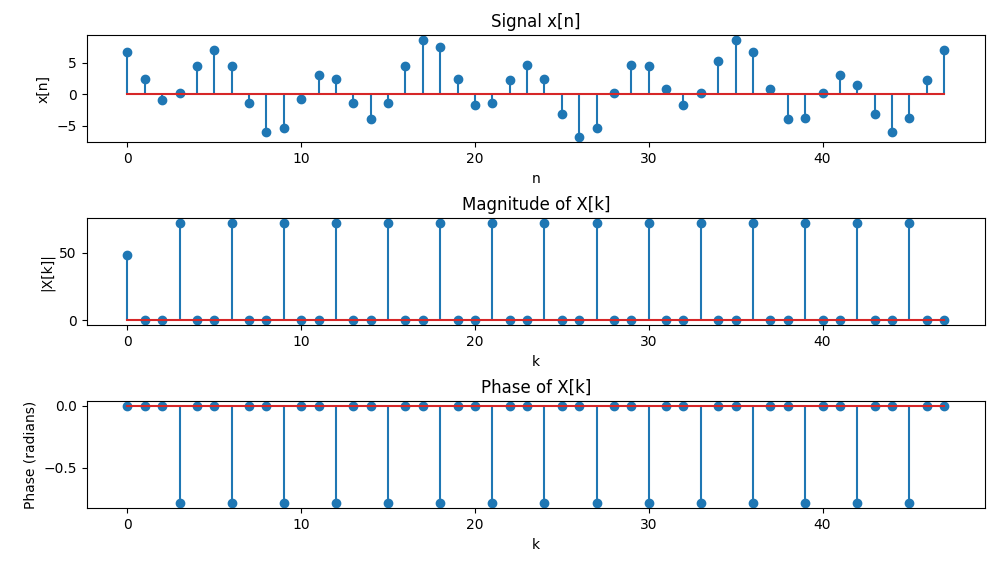
\includegraphics[width=\columnwidth]{2023/EE/49/figs/EE.49.png}
\end{figure}

%\end{document}










\newpage


\end{enumerate}
